\documentclass{article}
% =============================================================================
% Actionable Interpretability workshop @ COLM 2026.
%   Long track: <=9 pp main text, EXCLUDING references and appendix.
%   Double-blind (fully anonymized); non-archival; concurrent submission allowed.
% Anonymized via the colm2026_conference "submission" option (auto author block
%   + line numbers).  Body carries no author / repository / handle strings.
% =============================================================================
\usepackage[submission]{colm2026_conference}

\usepackage{microtype}
\usepackage{hyperref}
\usepackage{url}
\usepackage{booktabs}
\usepackage{amsmath,amssymb,amsfonts}
\usepackage{mathtools}
\usepackage{bm}
\usepackage{graphicx}
\usepackage{enumitem}
\usepackage{framed}
\usepackage{lineno}

\definecolor{darkblue}{rgb}{0, 0, 0.5}
\definecolor{shadecolor}{gray}{0.94}
\hypersetup{colorlinks=true, citecolor=darkblue, linkcolor=darkblue, urlcolor=darkblue}

% ---- notation ---------------------------------------------------------------
\newcommand{\R}{\mathbb{R}}
\DeclareMathOperator{\softmaxop}{softmax}
\newcommand{\softmax}{\softmaxop}
\DeclareMathOperator{\diagop}{diag}
\newcommand{\diag}{\diagop}
\DeclareMathOperator{\RMSNorm}{RMSNorm}
\newcommand{\dg}{\textsuperscript{$\dagger$}}

\title{Input-Affine Conditioning of Selective State-Space Models Is
Gauge-Absorbable:\\ A Diagnostic and a Design Rule}

\author{Anonymous Authors}

\begin{document}
\maketitle

\ifcolmsubmission
\linenumbers
\fi

\begin{abstract}
Selective state-space models (Mamba) have reshaped long-context sequence
modeling, yet which forms of conditioning \emph{survive} their training dynamics
is poorly understood---and getting it wrong is a quiet, recurring failure for
practitioners. We study FiLM-style regime conditioning of a Mamba backbone---a
per-block, channel-wise affine on each block's input, the natural drop-in way to
steer the input-dependent selective-scan parameters $\Delta,\mathbf{B},\mathbf{C}$---and
find it a \textbf{decisive null} with an \textbf{actionable} mechanistic
explanation. Under joint training the modulation collapses to identity and cannot
be forced active even by direct supervision. The reason is mechanical: an
input-side affine is a \textbf{gauge} direction that folds losslessly into the
block's own $\Delta/\mathbf{B}/\mathbf{C}$ projections, so the optimizer slides it
back to identity, with a dataset- and architecture-invariant signature
($\tau\approx7000$ steps, $R^2>0.999$) across FI-2010 equities, Kaggle crypto spot
books, and Polymarket prediction markets. An output-side placement sharpens rather
than escapes the mechanism---its scale folds into the block's \emph{other}
(bias-free output) projection and the one non-absorbable component, an additive
shift, decays in lockstep---so the null is \textbf{overdetermined}. This yields
actions a practitioner can take \emph{today} and a target for tomorrow. The
immediately usable parts are negative and diagnostic: do not expect input- or
output-affine regime conditioning of a selective scan to persist, and---before
crediting any conditioning---verify the gate is active with a \textbf{load-bearing
activation diagnostic} (an inert gate, $\mathrm{film}_g\!\approx\!0.004$--$0.010$
with $\mathrm{reg}_H$ at $\log R$, reported beside a positive generalization gap
means the gap is an \emph{artifact}, not a conditioning effect). The
\textbf{design rule} points further out: surviving conditioning must modulate
$\Delta/\mathbf{B}/\mathbf{C}$ \emph{inside} the fused kernel---a target we
validate at toy reference-scan scale, but one that needs a kernel-engineering
project to deploy, not a drop-in a practitioner can ship today. We package the
usable parts as a lift-and-use protocol, demonstrate the result on a financial
substrate with an architecture-agnosticism check (no backbone dominates), and
report a deflated economic coda for completeness.
\end{abstract}

\section{Introduction}\label{sec:intro}

Conditioning a network on side information---a task ID, a context vector, an
inferred regime---is among the most common things a practitioner does, and FiLM
(a channel-wise affine $\gamma\odot x+\beta$) \citep{perez2018film} is the
default mechanism. When the backbone is a \textbf{selective state-space model}
(Mamba \citep{gu2024mamba}), there is an especially tempting place to inject it.
Mamba's scan parameters $\Delta_t,\mathbf{B}_t,\mathbf{C}_t$ are
\emph{input-dependent} linear projections of each block's input, so an affine on
that input flows straight into the dynamics---and, crucially, it needs \textbf{no
change to the fused CUDA/TileLang kernel}. This is the drop-in form everyone
reaches for first. We show it does not work, explain mechanistically why, and
turn that explanation into two things a practitioner can use: a diagnostic that
catches a specific false-positive, and a design rule that says where a surviving
modulation has to live.

\paragraph{The finding.}
We introduce a \emph{RegimeFiLM} modulator that infers a categorical latent
regime and emits per-block affine parameters $(\gamma,\beta)$, zero-initialized so
the modulated backbone is \emph{exactly} the unmodulated baseline at step 0 (an
exact control). Despite the strongest activation pressure we could
apply---forced-active initialization plus direct supervision of the
router---the modulation decays to identity on every objective and dataset we test.
The cause is a \textbf{gauge symmetry}: a constant channel-wise scale on the block
input folds \emph{exactly} into the host projections $W_\Delta/W_B/W_C$ as a
right-multiplied diagonal $W_\bullet\diag(\gamma)$, and the shift folds into their
biases, with \textbf{no change to the function the block computes}. Identity is
therefore a flat, lossless valley the optimizer slides along; joint training
returns $(\gamma,\beta)\to(\mathbf{1},\mathbf{0})$. The decay constant is
dataset-invariant ($\tau\approx7000$, $R^2>0.999$) precisely because the
absorption direction is a property of the \emph{block parameterization}, not the
data. Moving the gate to the block \emph{output} does not escape this---the scale
folds into the bias-free output projection instead---so the null is overdetermined
by gauge absorption (every direction the host weights can represent) plus
reconstruction dominance (the one direction they cannot, the non-absorbable
shift, which simply earns nothing).

\paragraph{Why this is actionable.}
Two upshots change what a practitioner does.
\begin{itemize}[nosep,leftmargin=1.4em]
\item \emph{A diagnostic that catches a false-positive.} The activation
  diagnostics $\mathrm{film}_g=\mathrm{mean}\,|\gamma-1|$ and the router entropy
  $\mathrm{reg}_H$ (uniform maximum $\log R$) are \textbf{load-bearing}. In our
  data a generalization-gap metric reads \emph{positive}---with the ``right''
  sign---while FiLM is provably inert and the treatment is \emph{absolutely worse}
  in both regimes; the gap is a distributional ($\mathrm{high}-\mathrm{low}$)
  artifact whose sign even flips with head calibration. A practitioner who reports
  ``conditioning improved the out-of-regime gap'' without checking that the gate
  is actually \emph{on} can ship an artifact.
\item \emph{A design rule that says where to put the gate.} If you want regime
  conditioning of a selective scan to \emph{survive} training, the input-affine
  and output-affine forms will be folded back to identity. The surviving mechanism
  must act \textbf{between the block's bounding projections}---i.e., modulate
  $\Delta/\mathbf{B}/\mathbf{C}$ inside the fused kernel---or the conditioning
  should not be attempted in affine form at all. We delineate the boundary not as
  a parameterization that survives, but as the \emph{location} (inside the kernel)
  a surviving modulation would have to occupy.
\end{itemize}

\paragraph{Demonstration substrate.}
To stress the mechanism on genuinely different data we build a Mamba-3 world model
for limit-order-book (LOB) microstructure in the DreamerV3/Drama lineage
\citep{hafner2023dreamerv3, wang2024drama, lahoti2026mamba3}, exercised on FI-2010
equities, Kaggle crypto spot books, and Polymarket prediction markets
(\S\ref{sec:substrate}). The backbone is a substrate, not a claim: under matched
parameters \emph{no} backbone dominates across datasets
(\S\ref{sec:ablation})---exactly what a result about how selective scans
\emph{train}, rather than which one is best, should predict. The same study yields
a deflated economic coda (\S\ref{sec:coda}): conditioning the \emph{dynamics} did
not help, but a decision rule over the model's outputs is a survivable,
naive-beating edge that a logistic regression on the same features
reproduces---i.e., not attributable to the architecture. It is not the
contribution.

\section{Related Work}\label{sec:related}

\paragraph{Selective state-space models and Mamba.}
Structured state-space models (S4, S5, Mamba) give $O(n)$-complexity alternatives
to Transformers \citep{gu2022efficiently, smith2023s5, gu2024mamba}. Mamba
introduced \emph{selective} state spaces in which $\Delta$ and $\mathbf{B}$ are
input-dependent, enabling content-aware filtering; Mamba-2 \citep{dao2024mamba2}
formalized the duality with structured masked attention, and Mamba-3
\citep{lahoti2026mamba3} adds multi-input/multi-output (MIMO) transitions. The
property we exploit---that $\Delta_t,\mathbf{B}_t,\mathbf{C}_t$ are learned linear
projections of the block input---is exactly what makes an input-affine a gauge
direction. We are not aware of prior work characterizing the training-time fate of
FiLM-style conditioning of a selective scan.

\paragraph{FiLM and feature-wise conditioning.}
FiLM \citep{perez2018film} injects context as a channel-wise affine and is the
default conditioning primitive across vision, multi-task, and regime-embedding
settings \citep{lim2021time}. Our result is about \emph{where} in a selective-scan
block an affine can be placed and still survive joint training---a gauge
constraint specific to the input-dependent projection structure, orthogonal to
FiLM's expressive-power story.

\paragraph{Interpretability of training dynamics and weight symmetries.}
A line of interpretability work studies \emph{how} solutions form rather than
\emph{what} a fixed network computes, including reparameterization and gauge
symmetries that leave the function unchanged while reshaping the loss landscape
\citep{dinh2017sharp}. That a channel-wise affine before a linear map is redundant
with that map is a known theme in the normalization literature:
\citet{vanlaarhoven2017l2} shows weights feeding a normalization layer are
scale-invariant, so $L_2$ regularization acts on their \emph{scale}---and thus the
effective learning rate---rather than as capacity control, and
\citet{hoffer2018norm} and \citet{li2020exp} re-derive weight decay as an
effective-learning-rate schedule on the same symmetry. Our null is an instance of
this redundancy in a setting it has not been analyzed: the absorbed affine is not
a static normalization gain but a per-regime, \emph{input-dependent} FiLM that
folds into the selective scan's own $W_\Delta/W_B/W_C$ projections. What is new is
(i) the input-dependent selective-scan instantiation; (ii) the dataset- and
architecture-invariant decay signature ($\tau\approx7000$, $R^2>0.999$)
attributing the collapse to the optimizer; (iii) the output-side placement showing
the null is \emph{overdetermined} (gauge absorption plus reconstruction
dominance); and (iv) the practical consequence that the only kernel-friendly,
drop-in form is exactly the absorbable one---so the redundancy is the default a
practitioner reaches for, not a corner case. The actionable contribution is to
turn that symmetry into a measurable diagnostic ($\mathrm{film}_g$,
$\mathrm{reg}_H$) and a placement rule.

\paragraph{LOB models and regime-switching (substrate).}
DeepLOB \citep{zhang2019deeplob} and successors are discriminative LOB models on
FI-2010 \citep{ntakaris2018benchmark}; generative LOB work
\citep{nagy2023lobs5, backhouse2025painting} targets simulation fidelity;
classical regime-switching identifies discrete states from price processes
\citep{hamilton1989new}. We use these only as the demonstration substrate and
benchmark context, not as baselines for the conditioning result.

\section{Setup: FiLM Conditioning of a Selective Scan}\label{sec:setup}

\paragraph{Selective SSM.}
A discretized state-space layer maps $x_t\in\R^{d}$ to $y_t$ via a latent state
$h_t$: $h_t=\bar{\mathbf{A}}h_{t-1}+\bar{\mathbf{B}}x_t$, $y_t=\mathbf{C}h_t$.
Mamba makes the parameters \textbf{input-dependent}:
\begin{equation}\label{eq:selection}
\Delta_t=\sigma(W_\Delta\,x_t),\qquad \mathbf{B}_t=W_B\,x_t,\qquad
\mathbf{C}_t=W_C\,x_t,
\end{equation}
so \emph{any affine transformation of $x_t$ propagates directly into all three
scan parameters}. This is the selection mechanism we attempt to steer.

\paragraph{RegimeFiLM modulator.}
A regime head produces a soft categorical $\bm{\alpha}_t=\softmax(W_r\,x_t^{(0)})\in\R^R$
($R=8$) and a regime embedding $r_t=\bm{\alpha}_t^\top E$; a hypernetwork maps
$r_t$ to per-block affine parameters, bounded for bf16 stability:
\begin{equation}
\gamma^{(\ell)}=1+\tanh(\tilde{\gamma}^{(\ell)})\in(0,2),\qquad
\beta^{(\ell)}=\tanh(\tilde{\beta}^{(\ell)})\in(-1,1).
\end{equation}
The hypernetwork is \textbf{zero-initialized}, so at step 0
$\gamma^{(\ell)}=\mathbf{1},\beta^{(\ell)}=\mathbf{0}$ for all $\ell$ and the
modulated backbone is \emph{exactly} the unmodulated baseline---a clean, exact
paired control. A Switch-Transformer load-balancing term \citep{fedus2022switch}
maximizes the entropy of the \emph{batch-averaged} regime distribution,
$\mathcal{L}_{\text{regime}}=\lambda_{\text{ent}}(\log R-H[\bar{\bm{\alpha}}])$,
regularizing marginal usage while leaving per-step assignments free to be peaky.

\paragraph{Two application sites.}
The \textbf{input-affine} site routes the regime into the scan through the
selection mechanism:
\begin{equation}\label{eq:input}
x_t^{(\ell)}=x_t^{(\ell-1)}+\mathrm{Mamba3}\!\big(\gamma^{(\ell)}\odot\RMSNorm(x_t^{(\ell-1)})+\beta^{(\ell)}\big).
\end{equation}
As a control we also expose a \textbf{post-scan} site that gates the block
\emph{output}:
\begin{equation}\label{eq:postscan}
x_t^{(\ell)}=x_t^{(\ell-1)}+\gamma^{(\ell)}\odot\mathrm{Mamba3}\!\big(\RMSNorm(x_t^{(\ell-1)})\big)+\beta^{(\ell)}.
\end{equation}
Both share the identical modulator; only the site differs. This isolates the gauge
structure (\S\ref{sec:mechanism}): the input-side scale folds into
$W_\Delta/W_B/W_C$; the post-scan scale folds into the bias-free output projection
$W_{\text{out}}$; only the post-scan additive shift is non-absorbable.

\paragraph{Diagnostics.}
Activation metrics gate every claim:
$\mathrm{film}_g=\mathrm{mean}\,|\gamma-1|$ (deviation of the multiplicative gate
from identity), its additive counterpart $\mathrm{film}_b=\mathrm{mean}\,|\beta|$
(reported for the output-side shift in \S\ref{sec:gauge}), and the router entropy
$\mathrm{reg}_H$ (uniform maximum $\log R$, with $R$ the regime count; $\log 4$ on
FI-2010, $\log 8$ on Polymarket). \textbf{A positive generalization gap with an
inert FiLM is an artifact, not a regime-conditioning effect}---the central
methodological point.

\section{Demonstration Substrate (condensed)}\label{sec:substrate}

To exercise the mechanism on genuinely different distributions we instantiate the
modulated backbone inside a Mamba-3 world model for LOB microstructure
(DreamerV3/Drama lineage \citep{hafner2023dreamerv3, wang2024drama}): a
Transformer-over-depth encoder feeds a $16\times16$ categorical posterior and an
$L{=}4$ stack of Mamba-3 SISO blocks ($d_{\text{state}}{=}128$), trained with the
standard DreamerV3 loss (reconstruction $+$ dynamics/representation KL) plus light
auxiliary heads. The rest of the machinery (episodic memory, a Hawkes head, the
imagination loop, the EV-head internals) is in an accompanying codebase; no
conditioning result depends on any of it.

\paragraph{Regime axis.}
Beyond realized volatility we use a \textbf{predictability} axis on the underlying
spot series---Kaufman efficiency ratio
$\mathrm{ER}=|s_n-s_0|/\sum_t|s_t-s_{t-1}|$ (near 1 a clean trend, near 0 a random
wander), permutation entropy, and Hurst exponent---both to split the held-out
evaluation into forecastable vs.\ random-walk regimes and, when the router
collapses, to \emph{supervise it directly}. ``Is this window forecastable'' is the
most defensible regime signal we have; a router that will not encode even this axis
is the strongest form of the null.

\paragraph{Datasets.}
(i) Polymarket binary-outcome crypto LOBs (BTC/ETH/SOL up/down at 5/15/60-min
intervals, with the underlying Chainlink/Binance spot path); (ii) the public
FI-2010 benchmark \citep{ntakaris2018benchmark}; (iii) Kaggle high-frequency crypto
spot books (BTC/ETH/ADA at 1\,s / 1\,min / 5\,min). Held-out markets are split by
predictability (primary) and realized volatility (secondary), both reported.
\textbf{All thresholds are fit on the training split and frozen before any held-out
evaluation}, and baseline and treatment share the seed (an exact paired control).

\section{The Null and Its Mechanism}\label{sec:mechanism}

\subsection{RegimeFiLM is a decisive null}\label{sec:null}

Table~\ref{tab:film_null} reports the central diagnostic across five objectives
spanning two datasets and a money objective. In every family FiLM collapses to
identity under joint training: $\mathrm{film}_g$ decays toward zero and
$\mathrm{reg}_H$ sits at its uniform maximum ($\log R$). Where a generalization gap
reads positive (direction $+0.008$, settlement $+0.18$, by sign), FiLM is provably
inert, the treatment is \emph{absolutely worse} in both regimes, and the gap is a
$\mathrm{high}-\mathrm{low}$ distributional artifact whose sign even flips with head
calibration---which is exactly why the activation diagnostics are load-bearing. We
flag this against ourselves: read \emph{without} the gate diagnostic, both gaps
carry the sign a successful conditioner would produce, and we would have reported a
spurious win---it is only the inert $\mathrm{film}_g$ (with $\mathrm{reg}_H=\log R$)
that exposes the gap as an artifact. The false-positive is not a strawman; it is
the reading we ourselves nearly published.

\begin{table}[t]
\centering
\small
\begin{tabular}{lllrrl}
\toprule
Family & Objective & Dataset & Gap (sign, unit) & $\mathrm{film}_g$ & Verdict \\
\midrule
Volatility/scale & StudentT NLL    & FI-2010    & $\approx 0$ nats & $\approx$ ident.\ & \textsc{null} \\
Order-flow volume & Volume NLL     & FI-2010    & $\approx 0$ nats & $\approx$ ident.\ & \textsc{null} \\
Direction        & macro-F1        & FI-2010    & $+0.008$\dg\ F1 & $0.018$ & \textsc{null} \\
Settlement       & BCE log-loss    & Polymarket & $+0.18$\dg\ nats  & $0.008$ & \textsc{null} \\
\textbf{PnL}     & simulated trade & Polymarket & $-\$627$\dg   & $0.010$ & \textsc{null} \\
\bottomrule
\end{tabular}
\caption{RegimeFiLM is inert across every objective. $\mathrm{reg}_H$ equals its
uniform maximum ($\log R$) in all rows. The ``Gap'' column is in each objective's
own units (reconstruction NLL nats, macro-F1 points, BCE log-loss nats, dollars),
so its magnitude is not comparable across rows; only its sign and the inert
$\mathrm{film}_g$ are. \textsuperscript{$\dagger$}a non-zero gap whose sign is a
distributional artifact, not a FiLM effect (FiLM is inert, and the treatment is
absolutely worse). The PnL row's $-\$627$ is the FiLM A/B gap on the PnL
\emph{objective} (treatment$-$control), \emph{not} an economic total (cf.\ the
$+\$5{,}147$ settlement total in \S\ref{sec:coda}). The direction-row
$\mathrm{film}_g=0.018$ is the endpoint of the \emph{supervised} escalation on
that head (the joint-trained value is $\approx0.004$, cf.\
Table~\ref{tab:film_null_xdata}); the settlement ($0.008$) and PnL ($0.010$) rows
are joint-trained---all are inert, but the column mixes the two measurement
types.}
\label{tab:film_null}
\end{table}

\paragraph{Strongest-null test.}
Forcing FiLM active (zero-init scale raised so $\mathrm{film}_g=0.150$ at step 0)
and supervising the router \emph{directly} on the spot efficiency-ratio axis with
the strongest settings (LR multiplier 50, supervision weight 30, decoupled
router/FiLM, fed observation volatility) still decays the modulation monotonically
toward identity ($\mathrm{film}_g$:
$0.150\to0.119\to0.100\to0.074\to0.056\to0.043$, still falling) with
$\mathrm{reg}_H=\log 8$ throughout. The capacity is present but unused: a
\emph{frozen} router probes to $0.92$ agreement on the \emph{volatility}
bucket---the axis the representation encodes best---yet even there the modulation
collapses, while on the \emph{predictability} axis this escalation supervises the
regime decodes only weakly ($\approx0.25$--$0.36$).

\subsection{The mechanism: gauge absorption, and why it is overdetermined}\label{sec:gauge}

\paragraph{Cross-dataset invariance points at the optimizer.}
We take the architecture finding to FI-2010 (re-examined under the
predictability-primary axis) and the Kaggle crypto spot book (BTC/ETH/ADA at three
resolutions), judged by forecasting metrics alone. The zero-initialized modulation
never leaves identity: $\mathrm{film}_g\approx0.004$ and $\mathrm{reg}_H=\log 4$ in
every setting (Table~\ref{tab:film_null_xdata}). With FiLM an exact paired control,
every held-out gap is statistically indistinguishable from zero (all 95\% CIs
include 0) on both regime axes. The split is non-degenerate: high-efficiency-ratio
reference windows carry genuinely more structure on all three predictability
measures, and DeepLOB attains $0.628$ macro-F1 on the FI-2010 horizon-10
labels---so the null is a negative on \emph{forecastable} data, not a no-signal
artifact.

\begin{table}[t]
\centering
\small
\begin{tabular}{llrrl}
\toprule
Dataset & Asset / resolution & Gap (pred / vol) & $\mathrm{film}_g$ & Verdict \\
\midrule
FI-2010      & event stream          & $\approx 0$ / $\approx 0$ & $0.004$ & \textsc{null} \\
Kaggle BTC   & $1\,$min      & $\approx 0$ / $\approx 0$ & $0.004$ & \textsc{null} \\
Kaggle ETH   & $1\,$min      & $\approx 0$               & $0.005$ & \textsc{null} \\
Kaggle ADA   & $1\,$min      & $\approx 0$               & $0.005$ & \textsc{null} \\
Kaggle BTC   & $5\,$min      & $\approx 0$               & $0.005$ & \textsc{null} \\
Kaggle BTC   & $1\,$s (slice)& $\approx 0$               & $0.005$ & \textsc{null} \\
\bottomrule
\end{tabular}
\caption{Cross-dataset confirmation of the regime-FiLM null.
$\mathrm{reg}_H=\log 4$ (uniform router) in every row. The null is dataset-,
asset-, and resolution-independent.}
\label{tab:film_null_xdata}
\end{table}

\begin{figure}[t]
\centering

\includegraphics[width=0.74\linewidth]{figures/film_g_across_settings.pdf}
\caption{\textbf{RegimeFiLM is inert across every A/B setting}---the
gap-positive-but-gate-off diagnostic this paper is built on. The jointly-trained
treatment $\mathrm{film}_g=\mathrm{mean}\,|\gamma-1|$ (bars) sits near
$0.004$--$0.010$ on every dataset, asset, and resolution---FI-2010, Kaggle
BTC/ETH/ADA at three bar widths, and the two Polymarket objectives---while a
forced-active initialization starts at $0.150$ and the strongest-null escalation
at $0.250$ (dashed lines). The router entropy sits at its uniform maximum $\log R$
throughout. The modulation never grows from its exact identity initialization.}
\label{fig:film_across}
\end{figure}

\paragraph{The collapse is optimizer-driven.}
The predictability-supervised strongest-null test (forced-active FiLM, router
supervised directly on the efficiency-ratio bucket), applied at the
\textbf{input-side} gate, decays $\mathrm{film}_g$ monotonically at every logged
step on \emph{both} datasets (input-side: $0.250\to0.144$ Kaggle,
$0.250\to0.147$ FI-2010), with $\mathrm{reg}_H\approx\log 4$ throughout \emph{even
though the load-balance term is disabled}---so the uniform router is not a
load-balance artifact. An exponential fit $a\,e^{-t/\tau}+c$ matches both
trajectories at $R^2>0.999$ with near-identical parameters ($a\approx0.30$,
$\tau\approx7000$ steps). The decay is monotone with a negative slope sustained to
the last logged step (endpoint $\mathrm{film}_g\approx0.15$, still falling), and
the fitted asymptote lies at or below identity ($c\lesssim-0.05$, only more
negative when the lower bound on $c$ is relaxed), so the modulation extrapolates
toward identity rather than to a positive plateau---we rest the claim on the
observed monotone decay, with identity as the extrapolated limit. That the decay
rate is essentially \emph{identical} across two very different markets points at
the optimizer, not the data (Figure~\ref{fig:escalation_decay}).

\begin{figure}[t]
\centering

\includegraphics[width=0.60\linewidth]{figures/film_g_escalation_decay.pdf}
\caption{\textbf{Strongest-null test, and its placement-invariance.} Forcing the
modulation active ($\mathrm{film}_g=0.250$ at step 0) and supervising the router
directly on the efficiency-ratio bucket still decays $\mathrm{film}_g$
monotonically toward identity on both datasets (top, solid = \emph{input-side}
gate), with $\mathrm{reg}_H$ pinned at its uniform maximum $\log 4$ (bottom). An
exponential fit gives $R^2>0.999$ with a dataset-invariant time constant
$\tau\approx7000$ and a negative fitted asymptote, so the modulation extrapolates
toward identity rather than to a positive plateau. The \emph{output-side}
post-scan gate (top, dotted)
decays along the same trajectory---its scale folds into the bias-free output
projection just as the input-side scale folds into $W_\Delta/W_B/W_C$---so the null
is invariant to where the affine is applied. Endpoints differ only at the
round-off level by placement (input-side $0.250\!\to\!0.147$ FI-2010 /
$0.144$ Kaggle; output-side $0.250\!\to\!0.147$ FI-2010 / $0.143$ Kaggle, all at the
last logged step).}
\label{fig:escalation_decay}
\end{figure}

\paragraph{Why identity is a free direction: gauge absorption.}
Our modulation is an input-side affine, $\tilde{x}=\gamma\odot\hat{x}+\beta$,
applied to a block input that the very next operations re-project:
$\Delta_t=\sigma(W_\Delta\tilde{x}_t)$, $\mathbf{B}_t=W_B\tilde{x}_t$,
$\mathbf{C}_t=W_C\tilde{x}_t$. A constant channel-wise scale folds \emph{exactly}
into those projections as a right-multiplied diagonal, $W_\bullet\diag(\gamma)$,
and the shift folds into their biases, with \textbf{no change to the function the
block computes}; the host weights can thus represent any constant $(\gamma,\beta)$
themselves. Identity is therefore a \textbf{gauge} direction---a flat, lossless
valley the optimizer slides along---so joint training folds the modulation into the
host weights and returns $(\gamma,\beta)\to(\mathbf{1},\mathbf{0})$, which is
precisely the monotone decay we observe. This explains the dataset-invariant decay
constant (the absorption direction is a property of the block parameterization, not
the data) and \emph{scopes} the claim: \textbf{input-affine conditioning of a
selective scan is gauge-absorbable and will not persist under joint
training}---not that regime conditioning is impossible in principle. The fold is
exact for the \emph{constant} part of $\gamma$; the trained modulator is
input-dependent, but on a weakly-decodable regime the supervised router collapses to
uniform, $\gamma$ reduces to its constant part, and weight decay folds that to
identity---so the live mechanism reduces to the gauge one precisely when the regime
is hard to decode (the LM control below confirms the converse). The actionable
negative is that the most kernel-friendly, drop-in form of the idea is exactly the
form the optimizer can and does undo.

\paragraph{An output-side placement: the null is overdetermined.}
The gauge argument names an obvious next test---gating \emph{after} the scan---and
it does \emph{not} escape absorption. Each Mamba-3 block ends in a
\textbf{bias-free} output projection $y=W_{\text{out}}h$, so a channel-wise output
scale folds exactly into it,
$\gamma\odot(W_{\text{out}}h)=(\diag(\gamma)W_{\text{out}})h$---the same gauge move
on the block's \emph{other} face. The additive shift $\beta$ is different: with no
output bias and a nonlinear RMSNorm separating it from the next block, it is
genuinely \textbf{non-absorbable}. Under the identical forced-active escalation,
the output-side $\mathrm{film}_g$ and $\mathrm{film}_b$ decay in lockstep on both
datasets (output-side $\mathrm{film}_g$: $0.250\to0.147$ FI-2010,
$0.250\to0.143$ Kaggle), with the \emph{same} signature ($\tau\approx7065$ FI-2010
/ $6598$ Kaggle, $R^2>0.999$). The input- and output-side endpoints, read at the
same last logged step (FI-2010 $0.147$ vs.\ $0.147$; Kaggle $0.144$ vs.\ $0.143$),
differ only at round-off---placement changes \emph{nothing}, which is the point. The
null is therefore \textbf{overdetermined}---by two routes sharing a single driver,
weight decay over a loss that rewards neither: \textbf{gauge absorption} disposes of
every direction the
host weights can represent (the scale on \emph{either} face, hence the
placement-invariant constant), and \textbf{reconstruction dominance} disposes of
the one they cannot (the non-absorbable shift, killed because it earns nothing). A
modulation escaping both would have to act \emph{between} the block's bounding
projections---modulating $W_\Delta/W_B/W_C$ inside the fused kernel.

\paragraph{The boundary, demonstrated---and a gauge-vs-regularization control.}
Two cheap experiments turn the design rule from asserted to demonstrated.
\emph{(i) Folding.} On a toy reference scan, an input-affine modulation folds into
the host projections to floating-point precision (fold residual $1.2\times10^{-6}$,
the smallest deviation left after re-fitting the host projections to absorb the
forced-active gate) and decays to identity ($\mathrm{film}_g: 0.086\to0.010$), while
the \emph{same} modulation applied to $\Delta/\mathbf{B}/\mathbf{C}$ \emph{inside}
the scan is non-absorbable ($1.3\times10^{-2}$, $\sim10^4\times$ larger) and
\textbf{persists} ($0.093\to0.175$, seeds 0--3)---so the in-kernel target the rule
names is real. \emph{(ii) Weight-decay control.} Removing weight decay flattens the
decay ($\tau$ from $\approx6685$ to $\approx3\times10^5$, $R^2$ $0.9999\!\to\!0.48$),
so the gauge-direction decay is driven by \textbf{weight decay over a flat loss},
not the objective---and it is absent for the in-kernel placement.

\paragraph{When conditioning \emph{does} survive: regime decodability.}
The collapse is not universal, and the boundary is itself actionable. A Mamba
char-LM control on a two-domain corpus (English prose vs.\ Python source), with the
regime inferred by a context-aware router supervised on the domain and the
\emph{same} input-affine FiLM, does \textbf{not} collapse: with a strongly-decodable
regime (router $\sim0.95$ accuracy) $\mathrm{film}_g$ \emph{rises} from $0.11$ to
$0.52$. Gauge absorption always removes the \emph{constant} part of the affine; the
\emph{input-dependent} part survives only when the regime is decodable enough to be
worth encoding---in the LOB settings the regime is weakly decodable, the router
collapses to uniform, and the modulation reduces to its absorbable constant part.
\textbf{The actionable rule, refined:} skip the input-affine FiLM exactly when the
regime is weakly decodable from the block input; if it is strongly and contextually
decodable, the affine \emph{can} engage. (This control is a single-seed toy
experiment; the router$\Rightarrow$persistence outcome is clear, but the plateau
value $0.52$ is not load-bearing.)

\paragraph{The gap is real, and FiLM closes none of it.}
The null is not an absence of anything to fix: on the Kaggle book the high-volatility
windows are $+0.105$ worse in reconstruction NLL than the low-volatility windows in
\emph{both} arms, yet RegimeFiLM narrows the degradation by only $\sim0.001$ while
$\mathrm{film}_g$ is inert---it fails to engage a gap plainly present (linear-probe
localization in Appendix~\ref{app:probe}).

\subsection{Architecture-agnosticism check (matched-parameter backbone ablation)}\label{sec:ablation}

We compare Mamba-1, Mamba-2, Mamba-3 (SISO), and a Transformer-over-time under
matched parameter budgets ($\sim10.3$M) on FI-2010 and the Kaggle BTC spot book,
reporting held-out full-channel Student-$t$ reconstruction NLL (lower is better).
The result is a genuine ambiguity: \textbf{no backbone leads on both datasets}---Mamba-1
best on FI-2010, Mamba-2 (fewest SSM params) best on Kaggle, Mamba-3 SISO
competitive but not strictly dominant. A pre-norm Transformer matched to the
Mamba-3 block (RMSNorm, SiLU, $4\times$ FFN; $9.61$M) is likewise competitive but
non-dominant ($-0.5041$ FI-2010, $0.0224$ Kaggle), so the non-dominance is not an
artifact of an under-tuned post-norm baseline. This is exactly what a result about
how selective scans \emph{train}, rather than which one is best, should predict.

\begin{table}[t]
\centering
\small
\begin{tabular}{lrrr}
\toprule
Backbone & Params & FI-2010 recon NLL & Kaggle recon NLL \\
\midrule
Mamba-1                 & $11.45$M & $\mathbf{-0.5403}$ & $0.0241$ \\
Mamba-2                 & $10.20$M & $-0.5309$ & $\mathbf{-0.0213}$ \\
Mamba-3 SISO            & $10.30$M & $-0.5346$ & $0.0207$ \\
Transformer (post-norm) & $9.90$M  & $-0.5175$ & $0.0191$ \\
Transformer (pre-norm)  & $9.61$M  & $-0.5041$ & $0.0224$ \\
\bottomrule
\end{tabular}
\caption{Matched-parameter backbone ablation (held-out reconstruction NLL, lower
is better). No backbone wins both datasets, so the choice of sequence model is not
the operative variable.}
\label{tab:backbone}
\end{table}

\emph{Why SISO.} We run Mamba-3 in SISO throughout: the MIMO kernel's dynamic
shared-memory footprint exceeds the available GPU cap at every warp-valid
(rank, chunk) configuration, so the MIMO variant is outside this paper's hardware
envelope and we make no claim about it. This is the same kernel boundary the design
rule names---the surviving, in-kernel modulation of $\Delta/\mathbf{B}/\mathbf{C}$
lives behind the same fused-kernel wall.

\section{Deflated Economic Coda (substrate, one section)}\label{sec:coda}

The substrate yields a positive result the architecture did \emph{not} carry,
reported honestly as a deflated coda. Given the underlying spot path that
\textbf{defines} Polymarket settlement, the world model's directional settlement
probability---traded by a selective-participation strategy that bets only when a
train-frozen predictability gate fires---is a survivable, naive-beating edge whose
high-predictability slice a dependence-respecting market-block bootstrap (resampling
whole markets) places away from zero (95\% CI $[+\$2{,}445,\,+\$7{,}747]$ over $127$
markets, P(profit)$\approx1.0$). \textbf{Crucially the edge is
architecture-independent:} a logistic regression on the \emph{same} spot-conditioned
features, traded through the identical gate and engine, reproduces and \emph{exceeds}
it ($+\$6{,}914$ over $243$ markets vs.\ the settlement head's $+\$5{,}147$). Binary
settlement is a near-deterministic function of the spot move since open, so a linear
readout captures it at least as cleanly as the world model---the operative variable
is the spot-conditioned pipeline and the gate, \textbf{not the sequence model}. This
is the null's lesson from the other side: conditioning the \emph{dynamics} did not
help; a decision rule over the model's outputs did. The settlement head's marginal
low-predictability regime ($+\$51$, P$=0.63$), its tradeable-EV-head fix, the other
denominators, and the recorded-vintage reliability diagnostic are in
Appendix~\ref{app:coda}; the coda is not the contribution.

\section{Discussion: What a Practitioner Should Do Differently}\label{sec:discussion}

The interpretability finding is small and exact---an input-affine on a Mamba block
input is a gauge direction---but it has two consequences a practitioner can act on
immediately, which we package as the lift-and-use protocol below.

\begin{shaded}
\noindent\textbf{Diagnostic protocol: will my selective-scan conditioning
survive training?}\\[2pt]
\textbf{1. Instrument the gate.} Log $\mathrm{film}_g=\mathrm{mean}\,|\gamma-1|$
(deviation of the multiplicative gate from identity) and the router entropy
$\mathrm{reg}_H$ (uniform max $\log R$) at every checkpoint. \emph{Before} claiming
any conditioning ``helped,'' require $\mathrm{film}_g$ clearly $>0$ \emph{and}
$\mathrm{reg}_H$ off its uniform maximum. A positive generalization gap measured
against an inert gate ($\mathrm{film}_g\!\approx\!0$, $\mathrm{reg}_H\!=\!\log R$)
is a distributional artifact whose sign can flip with calibration---not a
conditioning effect.\\[2pt]
\textbf{2. Run the fold-residual placement test.} On a tiny reference scan, fit the
host projections to absorb a forced-active $(\gamma,\beta)$. Input- and
output-affine placements fold to round-off ($\sim\!10^{-6}$); a placement can
\emph{survive} only if its fold residual is large ($\sim\!10^{-2}$), i.e.\ it acts
on $\Delta/\mathbf{B}/\mathbf{C}$ \emph{between} the block's bounding projections
(inside the fused kernel).\\[2pt]
\textbf{3. Check regime decodability.} Affine conditioning engages only when the
regime is strongly decodable from the block input (router accuracy high,
$\mathrm{reg}_H$ low). If the router collapses to uniform, only the
gauge-absorbable constant remains---skip the affine.
\end{shaded}

\paragraph{Actionable takeaway.}
In one line: input- and output-affine FiLM of a Mamba selective scan are gauge
directions the optimizer folds back into the host
$\Delta/\mathbf{B}/\mathbf{C}$ (or bias-free output) projections and decays to
identity ($\tau\approx7000$, invariant across datasets and placement)---so
modulate $\Delta/\mathbf{B}/\mathbf{C}$ inside the fused kernel, or do not bother,
and verify the gate is on before reporting that conditioning ``helped.'' The
two-number check ($\mathrm{film}_g$, $\mathrm{reg}_H$) is cheap,
architecture-agnostic, and catches a seductive false-positive---an ablation that
``turns conditioning on'' and reports a better out-of-regime gap that moved for
distributional reasons while the conditioner never engaged.

\paragraph{The design rule names a target, not a dead end.}
What remains after gauge absorption and reconstruction dominance---modulating the
scan parameters \emph{between} the block's bounding projections, inside the fused
kernel---is the location a surviving modulation must occupy, and \S\ref{sec:gauge}
confirms at toy scale that a modulation placed there \emph{does} survive. That is a
kernel-engineering task (needing the shared-memory headroom the SISO/MIMO boundary
in \S\ref{sec:ablation} also runs into), and the natural next experiment.

\paragraph{Limitations.}
The decay is established at $\tau\approx7000$ over our training horizon; the
fitted asymptote lies at or below identity (robust to relaxing the lower bound on
$c$), so the modulation extrapolates \emph{through} identity, though the
within-horizon endpoint is still slightly above it---we do not claim a positive
near-identity plateau is impossible under every optimizer/schedule. The
constructive claims rest on single-seed toys (the LM control and the escalation
fits; the in-kernel toy is seeds 0--3), while the null is multi-setting and
multi-seed. The economic coda is a backtest substrate, not part of the
interpretability claim.

\section{Conclusion}\label{sec:conclusion}

An input-affine FiLM on a Mamba block input is a \textbf{gauge direction} the
optimizer folds back into the host projections, so it silently decays to identity
($\tau\approx7000$, $R^2>0.999$, invariant across datasets and placement); the null
is overdetermined by gauge absorption plus reconstruction dominance. What a
practitioner can act on \emph{today} is negative and diagnostic: do not ship input-
or output-affine regime conditioning of a selective scan, and verify the gate is on
(the two-number $\mathrm{film}_g/\mathrm{reg}_H$ check) before crediting it. The
constructive \textbf{design rule}---modulate $\Delta/\mathbf{B}/\mathbf{C}$ inside
the fused kernel---names the location a surviving modulation must occupy; we
validate it at toy scale and leave it as the next kernel-engineering step.

\appendix
\section{Deflated economic coda: figures}\label{app:coda}

\begin{figure}[h]
\centering
\begin{minipage}[t]{0.49\linewidth}\centering
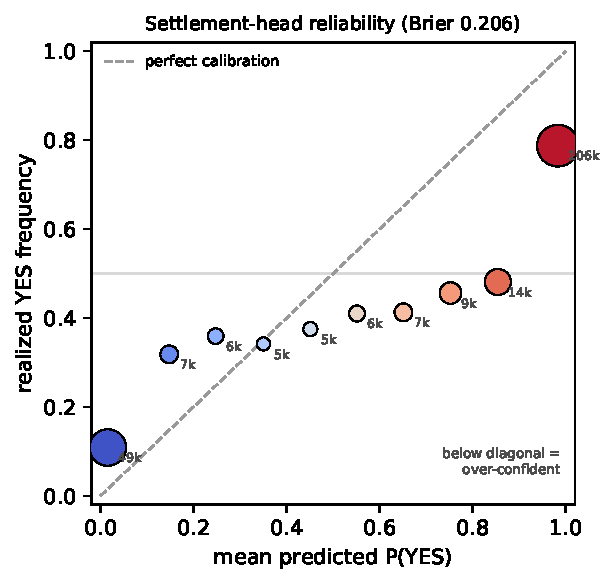
\includegraphics[width=\linewidth]{figures/reliability_settlement.pdf}
\end{minipage}\hfill
\begin{minipage}[t]{0.49\linewidth}\centering

\includegraphics[width=\linewidth]{figures/simple_baseline_pnl.pdf}
\end{minipage}
\caption{\textbf{Left:} settlement-head reliability over $214$k held-out
probabilities (Brier $0.206$). Points fall below the diagonal for mean $>0.5$
(systematic over-confidence), yet the populous extreme deciles land on the correct
side of $0.5$ ($0.787$ top decile, $0.109$ bottom decile; $0.785/0.108$ under
$0.1$-wide bins)---the directional signal the
divergence trade harvests; mid-confidence bins ($0.5$--$0.9$) realize below $0.5$,
the calibration footprint of the low-predictability failure the EV head removes.
\textbf{Right:} the economic edge does not need the architecture---held-out PnL of
the same-feature simple models on the $645$-market set, with market-block 95\% CIs.
The logistic's $+\$6{,}914$ exceeds both world-model heads, and its market-block
interval ($+\$2{,}844$ to $+\$10{,}880$ over $243$ independent markets) survives the
dependence-respecting bootstrap.}
\label{fig:coda}
\end{figure}

\paragraph{Economic-coda caveats (detail).}
The edge harvests the lag between the underlying spot and the contract book;
walk-the-book fills assume recorded liquidity is takeable, so live market impact
would erode some of it. Only the train-frozen predictability gate is
\emph{confirmatory}; the depth-band and early-market cuts are \emph{exploratory},
subject to forking-paths caveats. The reliability table and PnL totals are
recorded-vintage structural diagnostics---the over-confidence pattern is
structural, not vintage-specific.

\paragraph{Regime robustness via a tradeable-EV head (detail).}
Supervising the \emph{tradeable} expected value directly---a
\texttt{BookRelativeEdgeHead} trained with Huber loss on
$e_{\text{yes}}=\text{outcome}-\text{ask}_{\text{yes}}$,
$e_{\text{no}}=(1-\text{outcome})-\text{ask}_{\text{no}}$, so the target is near
zero (abstain) when the book is already fair---makes the low-predictability regime
robust: low-pred $+\$2{,}368$ at P(profit)$=0.99$ (seed 0); three-seed mean
$+\$4{,}779$ total at mean low-pred P(profit)$=0.98$, collapsing the high-vs-low PnL
spread $6.2\times$ ($\$5{,}044\to\$814$) at total PnL comparable to settlement
($+\$5{,}147$). The same-feature logistic is \emph{already} regime-robust---high-pred
$+\$2{,}448$, low-pred $+\$4{,}466$, both P(profit)$\ge0.99$---so the
low-predictability signal is not intrinsically hard; the EV head is a real fix
\emph{for the world-model readout}, not the only way to capture it.

\section{Linear-probe localization of regime decodability}\label{app:probe}

Two probes localize the failure behind the null. A post-hoc reading of the
jointly-supervised router shows it is uniform \emph{per step} (per-sample entropy
$\approx\log 4$) with near-chance agreement against the efficiency-ratio bucket
($0.25$--$0.31$ vs.\ $0.25$): direct supervision does not even make the router
regime-discriminative. A frozen linear probe on the unmodulated features decodes
the per-step predictability bucket only weakly ($0.33$--$0.36$ vs.\ $0.25$ chance)
and the volatility bucket somewhat better ($0.43$--$0.47$)---yet the volatility-axis
gap is \emph{also} null. So even on the axis the representation encodes best, and
even when the regime is supplied by supervision, the in-scan modulation collapses to
identity. (The degenerate next-tick direction head is de-confounded by
inverse-frequency class balancing, which yields a non-degenerate macro-F1 with the
gap still null; the single borderline gap, Kaggle spot-vol at $n{=}2$, is disproved
by a pre-registered third seed that flips its sign.)

\begin{thebibliography}{99}

\bibitem[Adams \& MacKay(2007)]{adams2007bayesian}
R.~P. Adams and D.~J.~C. MacKay.
\newblock Bayesian online changepoint detection.
\newblock \emph{arXiv preprint arXiv:0710.3742}, 2007.

\bibitem[Backhouse et~al.(2025)]{backhouse2025painting}
J.~Backhouse et~al.
\newblock Painting the market: Generative diffusion models for limit-order-book simulation and forecasting.
\newblock \emph{arXiv preprint arXiv:2509.05107}, 2025.

\bibitem[Dao \& Gu(2024)]{dao2024mamba2}
T.~Dao and A.~Gu.
\newblock Transformers are {SSMs}: Generalized models and efficient algorithms through structured state space duality.
\newblock In \emph{Proc.\ ICML}, 2024.

\bibitem[Dinh et~al.(2017)]{dinh2017sharp}
L.~Dinh, R.~Pascanu, S.~Bengio, and Y.~Bengio.
\newblock Sharp minima can generalize for deep nets.
\newblock In \emph{Proc.\ ICML}, 2017 (arXiv:1703.04933).

\bibitem[Fedus et~al.(2022)]{fedus2022switch}
W.~Fedus, B.~Zoph, and N.~Shazeer.
\newblock Switch {T}ransformers: Scaling to trillion parameter models with simple and efficient sparsity.
\newblock \emph{JMLR}, 23:1--39, 2022.

\bibitem[Gu et~al.(2022)]{gu2022efficiently}
A.~Gu, K.~Goel, and C.~R\'e.
\newblock Efficiently modeling long sequences with structured state spaces.
\newblock In \emph{Proc.\ ICLR}, 2022.

\bibitem[Gu \& Dao(2024)]{gu2024mamba}
A.~Gu and T.~Dao.
\newblock Mamba: Linear-time sequence modeling with selective state spaces.
\newblock In \emph{Proc.\ COLM}, 2024.

\bibitem[Hafner et~al.(2023)]{hafner2023dreamerv3}
D.~Hafner, J.~Pasukonis, J.~Ba, and T.~Lillicrap.
\newblock Mastering diverse domains through world models.
\newblock \emph{arXiv preprint arXiv:2301.04104}, 2023.

\bibitem[Hamilton(1989)]{hamilton1989new}
J.~D. Hamilton.
\newblock A new approach to the economic analysis of nonstationary time series and the business cycle.
\newblock \emph{Econometrica}, 57(2):357--384, 1989.

\bibitem[Hoffer et~al.(2018)]{hoffer2018norm}
E.~Hoffer, R.~Banner, I.~Golan, and D.~Soudry.
\newblock Norm matters: Efficient and accurate normalization schemes in deep networks.
\newblock In \emph{Proc.\ NeurIPS}, 2018 (arXiv:1803.01814).

\bibitem[Lahoti et~al.(2026)]{lahoti2026mamba3}
A.~Lahoti, K.~Y.~Li, B.~Chen, C.~Wang, A.~Bick, J.~Z.~Kolter, T.~Dao, and A.~Gu.
\newblock Mamba-3: Improved sequence modeling using state space principles.
\newblock In \emph{Proc.\ ICLR}, 2026 (arXiv:2603.15569).

\bibitem[Li \& Arora(2020)]{li2020exp}
Z.~Li and S.~Arora.
\newblock An exponential learning rate schedule for deep learning.
\newblock In \emph{Proc.\ ICLR}, 2020 (arXiv:1910.07454).

\bibitem[Lim et~al.(2021)]{lim2021time}
B.~Lim, S.~\"O. Arik, N.~Loeff, and T.~Pfister.
\newblock Temporal fusion transformers for interpretable multi-horizon time series forecasting.
\newblock \emph{International Journal of Forecasting}, 37(4):1748--1764, 2021.

\bibitem[Nagy et~al.(2023)]{nagy2023lobs5}
P.~Nagy, S.~Frey, S.~Sapora, K.~Li, A.~Calinescu, S.~Zohren, and J.~Foerster.
\newblock Generative {AI} for end-to-end limit order book modelling ({LOBS5}).
\newblock In \emph{Proc.\ ACM ICAIF}, 2023 (arXiv:2309.00638).

\bibitem[Ntakaris et~al.(2018)]{ntakaris2018benchmark}
A.~Ntakaris, M.~Magris, J.~Kanniainen, and M.~Gabbouj.
\newblock Benchmark dataset for mid-price forecasting of limit order book data with machine learning methods.
\newblock \emph{Journal of Forecasting}, 37(8):852--866, 2018.

\bibitem[Perez et~al.(2018)]{perez2018film}
E.~Perez, F.~Strub, H.~de~Vries, V.~Dumoulin, and A.~Courville.
\newblock {FiLM}: Visual reasoning with a general conditioning layer.
\newblock In \emph{Proc.\ AAAI}, 2018.

\bibitem[Smith et~al.(2023)]{smith2023s5}
J.~T.~H. Smith, A.~Warrington, and S.~W. Linderman.
\newblock Simplified state space layers for sequence modeling.
\newblock In \emph{Proc.\ ICLR}, 2023.

\bibitem[van Laarhoven(2017)]{vanlaarhoven2017l2}
T.~van Laarhoven.
\newblock {L2} regularization versus batch and weight normalization.
\newblock \emph{arXiv preprint arXiv:1706.05350}, 2017.

\bibitem[Wang et~al.(2024)]{wang2024drama}
W.~Wang et~al.
\newblock Drama: Mamba-enabled model-based reinforcement learning is sample and parameter efficient.
\newblock In \emph{Proc.\ ICLR}, 2025 (arXiv:2410.08893, 2024).

\bibitem[Zhang et~al.(2019)]{zhang2019deeplob}
Z.~Zhang, S.~Zohren, and S.~Roberts.
\newblock {DeepLOB}: Deep convolutional neural networks for limit order books.
\newblock \emph{IEEE Transactions on Signal Processing}, 67(11):3001--3012, 2019.

\end{thebibliography}

\end{document}
